
\section{Genotype likelihoods}

%%%%%%%%%%%%%%%%%%%%%%%%%%%%%%%%%%%%%%%%%%%%%%%%%
 
\frame{\frametitle{The data}

	\begin{figure}
		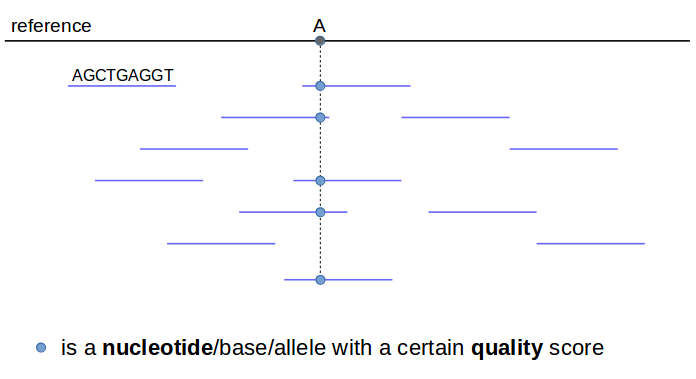
\includegraphics[scale=0.45]{Pics/mappedReads}
	\end{figure}

}

%%%%%%%%%%%%%%%%%%%%%%%%%%%%%%%%%%%%%%%%%%%%%%%%%%%%

\frame{\frametitle{Genotype likelihoods}

	\begin{block}{Likelihood}
		$P(D|G=\{A_1,A_2,...,A_n\})$
        \newline
		with
        \newline
		$A_i \in \{A,C,G,T\}$
        and $n$ being the ploidy
	\end{block}

How many genotypes likelihoods do we need to calculate for each each individual at each site?

}

%%%%%%%%%%%%%%%%%%%%%%%%%%%%%%%%%%%%%%%%%%%%%%%%%%%%

\frame{\frametitle{Genotype likelihoods}

	\begin{figure}
		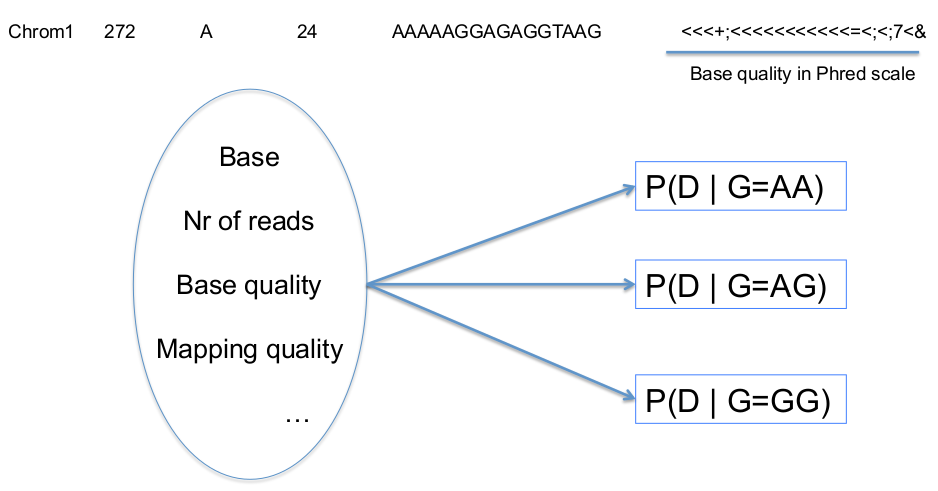
\includegraphics[scale=0.3]{Pics/genoLikes}
	\end{figure}

}


%%%%%%%%%%%%%%%%%%%%%%%%%%%%%%%%%%%%%%%%%%%%%%%%%%%%

\frame{\frametitle{Calculating genotype likelihoods}

\begin{block}{Likelihood function}

	\begin{equation*}
		P(D|G=\{A_1,A_2,...,A_N\}) = \prod_{i=1}^R \sum_{j=1}^N \frac{L_{A_j,i}}{N}
	\end{equation*}
 
 	\begin{itemize}
    	\item $L_{A_j,i} = P(D|A_G=A_j)$
    	\item $A_i \in \{A,C,G,T\}$
		\item $R$ is the depth (nr. of reads)
    	\item $N$ is the ploidy (nr. of chromosomes)
	\end{itemize}
    
\end{block}

Example: 
\newline
AAAG with all quality scores equal to 20 (in phred score)
\newline
$P(D|G=AC) = ?$

}


%%%%%%%%%%%%%%%%%%%%%%%%%%%%%%%%%%%%%%%%%%%%%%%%%%%%

\frame{\frametitle{Calculating genotype likelihoods}

	\begin{block}{Likelihood function}

		\begin{equation*}
			P(D|G=\{A_1,A_2,...,A_N\}) = \prod_{i=1}^R \sum_{j=1}^N \frac{L_{A_j,i}}{N}
		\end{equation*}
  
	\end{block}

	AAAG \& Q=20

	\begin{equation*}
		P(D|G=\{A,C\}) = ...
	\end{equation*}

}

%%%%%%%%%%%%%%%%%%%%%%%%%%%%%%%%%%%%%%%%%%%%%%%%%%%%%%%%%%%%%%%%%%%%

\frame{\frametitle{Calculating genotype likelihoods}

	\begin{block}{Likelihood function}

		\begin{equation*}
			P(D|G=\{A_1,A_2,...,A_N\}) = \prod_{i=1}^R \sum_{j=1}^N \frac{L_{A_j,i}}{N}
		\end{equation*}
  
	\end{block}

	AAAG \& Q=20

	$N=2; i=1; A_1=A; A_2=C$

	\begin{equation*}
		P(D|G=\{A,C\}) = (\frac{L_{A,1}}{2} + \frac{L_{C,1}}{2}) \times ...
	\end{equation*}

	What are $L_{A,1}$ and $L_{C,1}$?

}

%%%%%%%%%%%%%%%%%%%%%%%%%%%%%%%%%%%%%%%%%%%%%%%%%%%%%%%%%%%%%%%%%%%%

\frame{\frametitle{Calculating genotype likelihoods}

	\begin{block}{Likelihood function}

		\begin{equation*}
			P(D|G=\{A_1,A_2,...,A_N\}) = \prod_{i=1}^R \sum_{j=1}^N \frac{L_{A_j,i}}{N}
		\end{equation*}
  
	\end{block}

	AAAG \& Q=20

	\begin{equation*}
			L_{C,1} = \frac{\epsilon}{3}	
	\end{equation*}

	\begin{equation*}
    	L_{A,1} = 1-\epsilon
	\end{equation*}
    
	\begin{equation*}
		P(D|G=\{A,C\}) = (\frac{1-\epsilon}{2} + \frac{\epsilon}{6}) \times ...
	\end{equation*}



}

%%%%%%%%%%%%%%%%%%%%%%%%%%%%%%%%%%%%%%%%%%%%%%%%%%%%%%%%%%%%%%%%%%%%

\frame{\frametitle{Calculating genotype likelihoods}

	\begin{block}{Likelihood function}

		\begin{equation*}
			P(D|G=\{A_1,A_2,...,A_N\}) = \prod_{i=1}^R \sum_{j=1}^N \frac{L_{A_j,i}}{N}
		\end{equation*}
  
	\end{block}

	AAAG \& Q=20

	\begin{equation*}
			L_{C,1} = \frac{\epsilon}{3}	
	\end{equation*}

	\begin{equation*}
    	L_{A,1} = 1-\epsilon
	\end{equation*}
    
	\begin{equation*}
		P(D|G=\{A,C\}) = (\frac{1-\epsilon}{2} + \frac{\epsilon}{6}) \times \frac{\epsilon}{3} \times \frac{\epsilon}{3} \times \frac{\epsilon}{3}
	\end{equation*}

	What is $\epsilon$?

}

%%%%%%%%%%%%%%%%%%%%%%%%%%%%%%%%%%%%%%%%%%%%%%%%%%%%%%%%%%%%%%%%%%%%

\frame{\frametitle{Calculating genotype likelihoods}

	\begin{columns}
	
    	\column{0.6\textwidth}   

		\begin{center}
			\begin{tabular}{c | c}
			Genotype & Likelihood (log10)\\
    		\hline
	    	AA & -2.49\\
    		\textbf{AC} & \textbf{-3.38}\\
    		AG & -1.22\\
    		AT & -3.38\\
            CC & -9.91\\
            CG & -7.74\\
            CT & -9.91\\
            GG & -7.44\\
            GT & -7.74\\
            TT & -9.91\\
        	\hline
			\end{tabular}
       	\end{center}

		\column{0.4\textwidth}

		AAAG \& $\epsilon=0.01$

	\end{columns}


}

